\begin{figure}[htbp]
\centering
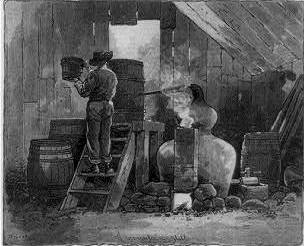
\includegraphics[width=.4\textwidth]{../pictures/moonshine.jpg}
\end{figure}

\subsubsection{Peering into Learning}

\noindent This is a quick introduction to the main ideas used in the rest of the
book. It provides a range of things to think about as you get started
with a new peer learning project, or as you use peeragogy to redesign
and reassess an existing collaboration. You'll probably want to read
this first and then do some reflection before diving into the other
parts of the book.

\subsubsection{Motivation}
You might wonder why we're doing this project -- what we hope to get
out of it as volunteers, and how we think what we're doing can make a
positive difference in the world. Have a look at this chapter if you,
too, are thinking about getting involved in peeragogy, or wondering
how peeragogy can help you accelerate your own learning projects.

\paragraph{Case Study: 5PH1NX}
We enjoy riddles with more than one answer, so we've included this
detailed narrative example of peeragogy in action near the beginning
of the book. We hope you are inspired by the challenge of doing
peeragogy in a school setting that is recounted here. Explore this
case study for ideas and encouragement for your own learning
adventures.

\subsubsection{Patterns, use cases, examples}

\noindent Here we show you some of the signposts that can serve as
both a key and compass to the kind of social problem solving that
happens in peeragogy projects. If you want some underlying components
to try out, mix and match these and experiment with peeragogy right
away. You come back to this chapter for a deeper understanding of the
processes we talk about later on. A detailed catalog of patterns and
anti-patterns that we've drawn from our own practice form a core part
of the book.

\subsubsection{Convening a Group}

\noindent You'll probably want to use this chapter to organize your thinking as
you start a new peeragogy project or think about how to apply peeragogy
ideas in an existing collaboration. A few clusters of simple but
important questions will inspire unique answers for you and your group.
We hope these mental frameworks are helpful to not only initiate
progress, but also to maintain momentum.

 \paragraph{Play \& Learning} What
makes learning fun? Just as actors learn their roles through the dynamic
process of performance, In other words, the more we engage with a topic,
the better we learn it and the more satisfying - or fun - the process
becomes.

\paragraph{K-12 Peeragogy} The key to becoming a successful
`connected educator-learner' involves spending the time needed to learn
how to learn and share in an open, connected environment. Once you make
the decision to enter into a dialogue with another user, you become a
connected educator/learner and tap into the power of networks to
distribute the load of learning. Depending on their age, you can even
facilitate an awareness of peer networks among your students.

\paragraph{P2P Self-Organizing Learning Environments} This conversational
section engages you in a journey through diverse points of entry that
interact with your physical learning space. Within this chapter of word
and picture images, the emerging structure and reciprocal mentoring that
may be inspired causes a ripple effect on those who open the door to its
possibilities.

\subsubsection{Organizing a Learning Context}

\noindent We talk about how peer learning is organized into ``courses'' and
``spaces'', again drawing on our experience in the peeragogy project. We
present the results of an informal poll that reveals some of the
positive and some of the negative features of our early choices.

\paragraph{Adding Structure with Activities} The first rule of thumb for
peer learning is: announce activities only when you plan to take part as
a fully engaged participant. Then ask a series of questions: what is the
goal, what makes it challenging, what worked in other situations, what
recipe is appropriate, what is different about learning about this
topic?

\paragraph{Student Authored Syllabus} Here's one place you might
explore to see ways in which freedom in student-directed learning
complements the structural needs for the content and group. Check this
out for various methods to welcome ambiguity and co-created curriculum
into your projects. You may want to start with one or two ideas in an
activity to transition into this format, yet embracing the risk on a
larger scale is fun as well.

\paragraph{Connectivism in Practice} Massive Open
Online Courses (MOOCs) are decentralized online learning experiences:
individuals and groups create blogs or wikis and comment on each
other's work, often with a focus on where to find information. A
course typically has a topic, activities, reading resources and a
guest speaker for each week. Items are tagged to allow for
aggregation. Links to technology resources are provided (such as
gRSShopper from Stephen Downes).

\paragraph{Case Study: Collaborative Explorations} You can try out this
chapter to encourage individuals pursuing their own interests in a
predetermined topic while at the same time influencing the learning of
the whole group by sharing and reflecting upon their findings. These
interactions of supportive mutual inquiry evolve the content and
structure within a short time frame and with open-ended results.

\subsubsection{Cooperation}

\noindent Sometimes omitting the figurehead empowers a
group. Co-facilitation tends to work in groups of people who gather to
share common problems and experiences. The chapter suggests how to
co-facilitate discussions, wiki workflows, and live
sessions. Conducting an ``after action review'' helps to avoid blind
spots.

\paragraph{The Workscape} In a corporate workscape, people are free-range
learners: protect the learning environment, provide nutrients for
growth, and let nature take its course. A workscape features profiles,
an activity stream, wikis, virtual meetings, blogs, bookmarks, mobile
access and a social network.

\paragraph{Participation} Participation grows from having a
community of people who learn together, using a curriculum as a starting
point to organize and trigger engagement. Keep in mind that
participation may follow the 90/9/1 principle (lurkers/editors/authors)
and that people may transition through these roles over time.

\paragraph{New Designs For Co-Working And Co-Learning} Designing for
peer learning requires a new approach.  A case study dealing focusing
on PlanetMath shows one way to go.

\subsubsection{Assessment}

\noindent Asking questions about assessment in the context of the
Handbook (Who needs to know? Based on what data? In what format?)
suggests ``usefulness'' (real problems solved) is an appropriate
metric. We use the idea of return on investment (the value of changes
in behavior divided by the cost of inducing the change) to assess the
peeragogy project itself, as one example.

\paragraph{Researching peeragogy} Three new patterns are introduced
(Frontend and Backend, Spanning Set, and Minimum Viable Project) which
form the basis of a ``meta-model'' that can be used to study and
design for peer learning.

\subsubsection{Technologies, Services, and Platforms}

\noindent Issues of utility, choice, coaching, impact and roles attach
to the wide variety of tools and technologies available for peer
learning. Keys to selection include the features you need, what people
are already using, and the type of tool (low threshold, wide wall,
high ceilings) used for collaboration.

\paragraph{Forums} Forums are web-based communication media
that enable groups of people to conduct organized multimedia discussions
about multiple topics over a period of time, asynchronously. A rubric
for evaluating forum posts highlights the value of drawing connections.
The chapter includes tips on selecting forum software.

\paragraph{Wiki} A
wiki is a website whose users can add, modify, or delete its content via
a web browser. Pages have a feature called ``history'' which allows
users to see previous versions and roll back to them. The chapter
includes tips on how to use a wiki and select a wiki engine, with
particular attention to peer learning opportunities.

 \paragraph{Real-time meetings} Web services enable broadband-connected
learners to communicate in real time via audio, video, slides,
whiteboards, chat, and screen-sharing. Possible roles for participants
in real-time meetings include searchers, contextualizers, summarizers,
lexicographers, mappers, and curators. This mode of interaction
supports emergent agendas.

\subsubsection{Resources}

\noindent Here we present several ways to get involved in peer
learning, including information about where to find the Peeragogy
project online, a sample syllabus with four actions bring peer
learning to life, tips on writing for The Handbook, and our Creative
Commons Zero 1.0 Universal (CC0 1.0) Public Domain Dedication.
